\documentclass[11pt]{article}

    \usepackage[breakable]{tcolorbox}
    \usepackage{parskip} % Stop auto-indenting (to mimic markdown behaviour)
    

    % Basic figure setup, for now with no caption control since it's done
    % automatically by Pandoc (which extracts ![](path) syntax from Markdown).
    \usepackage{graphicx}
    % Keep aspect ratio if custom image width or height is specified
    \setkeys{Gin}{keepaspectratio}
    % Maintain compatibility with old templates. Remove in nbconvert 6.0
    \let\Oldincludegraphics\includegraphics
    % Ensure that by default, figures have no caption (until we provide a
    % proper Figure object with a Caption API and a way to capture that
    % in the conversion process - todo).
    \usepackage{caption}
    \DeclareCaptionFormat{nocaption}{}
    \captionsetup{format=nocaption,aboveskip=0pt,belowskip=0pt}

    \usepackage{float}
    \floatplacement{figure}{H} % forces figures to be placed at the correct location
    \usepackage{xcolor} % Allow colors to be defined
    \usepackage{enumerate} % Needed for markdown enumerations to work
    \usepackage{geometry} % Used to adjust the document margins
    \usepackage{amsmath} % Equations
    \usepackage{amssymb} % Equations
    \usepackage{textcomp} % defines textquotesingle
    % Hack from http://tex.stackexchange.com/a/47451/13684:
    \AtBeginDocument{%
        \def\PYZsq{\textquotesingle}% Upright quotes in Pygmentized code
    }
    \usepackage{upquote} % Upright quotes for verbatim code
    \usepackage{eurosym} % defines \euro

    \usepackage{iftex}
    \ifPDFTeX
        \usepackage[T1]{fontenc}
        \IfFileExists{alphabeta.sty}{
              \usepackage{alphabeta}
          }{
              \usepackage[mathletters]{ucs}
              \usepackage[utf8x]{inputenc}
          }
    \else
        \usepackage{fontspec}
        \usepackage{unicode-math}
    \fi

    \usepackage{fancyvrb} % verbatim replacement that allows latex
    \usepackage{grffile} % extends the file name processing of package graphics
                         % to support a larger range
    \makeatletter % fix for old versions of grffile with XeLaTeX
    \@ifpackagelater{grffile}{2019/11/01}
    {
      % Do nothing on new versions
    }
    {
      \def\Gread@@xetex#1{%
        \IfFileExists{"\Gin@base".bb}%
        {\Gread@eps{\Gin@base.bb}}%
        {\Gread@@xetex@aux#1}%
      }
    }
    \makeatother
    \usepackage[Export]{adjustbox} % Used to constrain images to a maximum size
    \adjustboxset{max size={0.9\linewidth}{0.9\paperheight}}

    % The hyperref package gives us a pdf with properly built
    % internal navigation ('pdf bookmarks' for the table of contents,
    % internal cross-reference links, web links for URLs, etc.)
    \usepackage{hyperref}
    % The default LaTeX title has an obnoxious amount of whitespace. By default,
    % titling removes some of it. It also provides customization options.
    \usepackage{titling}
    \usepackage{longtable} % longtable support required by pandoc >1.10
    \usepackage{booktabs}  % table support for pandoc > 1.12.2
    \usepackage{array}     % table support for pandoc >= 2.11.3
    \usepackage{calc}      % table minipage width calculation for pandoc >= 2.11.1
    \usepackage[inline]{enumitem} % IRkernel/repr support (it uses the enumerate* environment)
    \usepackage[normalem]{ulem} % ulem is needed to support strikethroughs (\sout)
                                % normalem makes italics be italics, not underlines
    \usepackage{soul}      % strikethrough (\st) support for pandoc >= 3.0.0
    \usepackage{mathrsfs}
    

    
    % Colors for the hyperref package
    \definecolor{urlcolor}{rgb}{0,.145,.698}
    \definecolor{linkcolor}{rgb}{.71,0.21,0.01}
    \definecolor{citecolor}{rgb}{.12,.54,.11}

    % ANSI colors
    \definecolor{ansi-black}{HTML}{3E424D}
    \definecolor{ansi-black-intense}{HTML}{282C36}
    \definecolor{ansi-red}{HTML}{E75C58}
    \definecolor{ansi-red-intense}{HTML}{B22B31}
    \definecolor{ansi-green}{HTML}{00A250}
    \definecolor{ansi-green-intense}{HTML}{007427}
    \definecolor{ansi-yellow}{HTML}{DDB62B}
    \definecolor{ansi-yellow-intense}{HTML}{B27D12}
    \definecolor{ansi-blue}{HTML}{208FFB}
    \definecolor{ansi-blue-intense}{HTML}{0065CA}
    \definecolor{ansi-magenta}{HTML}{D160C4}
    \definecolor{ansi-magenta-intense}{HTML}{A03196}
    \definecolor{ansi-cyan}{HTML}{60C6C8}
    \definecolor{ansi-cyan-intense}{HTML}{258F8F}
    \definecolor{ansi-white}{HTML}{C5C1B4}
    \definecolor{ansi-white-intense}{HTML}{A1A6B2}
    \definecolor{ansi-default-inverse-fg}{HTML}{FFFFFF}
    \definecolor{ansi-default-inverse-bg}{HTML}{000000}

    % common color for the border for error outputs.
    \definecolor{outerrorbackground}{HTML}{FFDFDF}

    % commands and environments needed by pandoc snippets
    % extracted from the output of `pandoc -s`
    \providecommand{\tightlist}{%
      \setlength{\itemsep}{0pt}\setlength{\parskip}{0pt}}
    \DefineVerbatimEnvironment{Highlighting}{Verbatim}{commandchars=\\\{\}}
    % Add ',fontsize=\small' for more characters per line
    \newenvironment{Shaded}{}{}
    \newcommand{\KeywordTok}[1]{\textcolor[rgb]{0.00,0.44,0.13}{\textbf{{#1}}}}
    \newcommand{\DataTypeTok}[1]{\textcolor[rgb]{0.56,0.13,0.00}{{#1}}}
    \newcommand{\DecValTok}[1]{\textcolor[rgb]{0.25,0.63,0.44}{{#1}}}
    \newcommand{\BaseNTok}[1]{\textcolor[rgb]{0.25,0.63,0.44}{{#1}}}
    \newcommand{\FloatTok}[1]{\textcolor[rgb]{0.25,0.63,0.44}{{#1}}}
    \newcommand{\CharTok}[1]{\textcolor[rgb]{0.25,0.44,0.63}{{#1}}}
    \newcommand{\StringTok}[1]{\textcolor[rgb]{0.25,0.44,0.63}{{#1}}}
    \newcommand{\CommentTok}[1]{\textcolor[rgb]{0.38,0.63,0.69}{\textit{{#1}}}}
    \newcommand{\OtherTok}[1]{\textcolor[rgb]{0.00,0.44,0.13}{{#1}}}
    \newcommand{\AlertTok}[1]{\textcolor[rgb]{1.00,0.00,0.00}{\textbf{{#1}}}}
    \newcommand{\FunctionTok}[1]{\textcolor[rgb]{0.02,0.16,0.49}{{#1}}}
    \newcommand{\RegionMarkerTok}[1]{{#1}}
    \newcommand{\ErrorTok}[1]{\textcolor[rgb]{1.00,0.00,0.00}{\textbf{{#1}}}}
    \newcommand{\NormalTok}[1]{{#1}}

    % Additional commands for more recent versions of Pandoc
    \newcommand{\ConstantTok}[1]{\textcolor[rgb]{0.53,0.00,0.00}{{#1}}}
    \newcommand{\SpecialCharTok}[1]{\textcolor[rgb]{0.25,0.44,0.63}{{#1}}}
    \newcommand{\VerbatimStringTok}[1]{\textcolor[rgb]{0.25,0.44,0.63}{{#1}}}
    \newcommand{\SpecialStringTok}[1]{\textcolor[rgb]{0.73,0.40,0.53}{{#1}}}
    \newcommand{\ImportTok}[1]{{#1}}
    \newcommand{\DocumentationTok}[1]{\textcolor[rgb]{0.73,0.13,0.13}{\textit{{#1}}}}
    \newcommand{\AnnotationTok}[1]{\textcolor[rgb]{0.38,0.63,0.69}{\textbf{\textit{{#1}}}}}
    \newcommand{\CommentVarTok}[1]{\textcolor[rgb]{0.38,0.63,0.69}{\textbf{\textit{{#1}}}}}
    \newcommand{\VariableTok}[1]{\textcolor[rgb]{0.10,0.09,0.49}{{#1}}}
    \newcommand{\ControlFlowTok}[1]{\textcolor[rgb]{0.00,0.44,0.13}{\textbf{{#1}}}}
    \newcommand{\OperatorTok}[1]{\textcolor[rgb]{0.40,0.40,0.40}{{#1}}}
    \newcommand{\BuiltInTok}[1]{{#1}}
    \newcommand{\ExtensionTok}[1]{{#1}}
    \newcommand{\PreprocessorTok}[1]{\textcolor[rgb]{0.74,0.48,0.00}{{#1}}}
    \newcommand{\AttributeTok}[1]{\textcolor[rgb]{0.49,0.56,0.16}{{#1}}}
    \newcommand{\InformationTok}[1]{\textcolor[rgb]{0.38,0.63,0.69}{\textbf{\textit{{#1}}}}}
    \newcommand{\WarningTok}[1]{\textcolor[rgb]{0.38,0.63,0.69}{\textbf{\textit{{#1}}}}}


    % Define a nice break command that doesn't care if a line doesn't already
    % exist.
    \def\br{\hspace*{\fill} \\* }
    % Math Jax compatibility definitions
    \def\gt{>}
    \def\lt{<}
    \let\Oldtex\TeX
    \let\Oldlatex\LaTeX
    \renewcommand{\TeX}{\textrm{\Oldtex}}
    \renewcommand{\LaTeX}{\textrm{\Oldlatex}}
    % Document parameters
    % Document title
    \title{schuler\_5779\_ece\_527\_report\_03}
    
    
    
    
    
    
    
% Pygments definitions
\makeatletter
\def\PY@reset{\let\PY@it=\relax \let\PY@bf=\relax%
    \let\PY@ul=\relax \let\PY@tc=\relax%
    \let\PY@bc=\relax \let\PY@ff=\relax}
\def\PY@tok#1{\csname PY@tok@#1\endcsname}
\def\PY@toks#1+{\ifx\relax#1\empty\else%
    \PY@tok{#1}\expandafter\PY@toks\fi}
\def\PY@do#1{\PY@bc{\PY@tc{\PY@ul{%
    \PY@it{\PY@bf{\PY@ff{#1}}}}}}}
\def\PY#1#2{\PY@reset\PY@toks#1+\relax+\PY@do{#2}}

\@namedef{PY@tok@w}{\def\PY@tc##1{\textcolor[rgb]{0.73,0.73,0.73}{##1}}}
\@namedef{PY@tok@c}{\let\PY@it=\textit\def\PY@tc##1{\textcolor[rgb]{0.24,0.48,0.48}{##1}}}
\@namedef{PY@tok@cp}{\def\PY@tc##1{\textcolor[rgb]{0.61,0.40,0.00}{##1}}}
\@namedef{PY@tok@k}{\let\PY@bf=\textbf\def\PY@tc##1{\textcolor[rgb]{0.00,0.50,0.00}{##1}}}
\@namedef{PY@tok@kp}{\def\PY@tc##1{\textcolor[rgb]{0.00,0.50,0.00}{##1}}}
\@namedef{PY@tok@kt}{\def\PY@tc##1{\textcolor[rgb]{0.69,0.00,0.25}{##1}}}
\@namedef{PY@tok@o}{\def\PY@tc##1{\textcolor[rgb]{0.40,0.40,0.40}{##1}}}
\@namedef{PY@tok@ow}{\let\PY@bf=\textbf\def\PY@tc##1{\textcolor[rgb]{0.67,0.13,1.00}{##1}}}
\@namedef{PY@tok@nb}{\def\PY@tc##1{\textcolor[rgb]{0.00,0.50,0.00}{##1}}}
\@namedef{PY@tok@nf}{\def\PY@tc##1{\textcolor[rgb]{0.00,0.00,1.00}{##1}}}
\@namedef{PY@tok@nc}{\let\PY@bf=\textbf\def\PY@tc##1{\textcolor[rgb]{0.00,0.00,1.00}{##1}}}
\@namedef{PY@tok@nn}{\let\PY@bf=\textbf\def\PY@tc##1{\textcolor[rgb]{0.00,0.00,1.00}{##1}}}
\@namedef{PY@tok@ne}{\let\PY@bf=\textbf\def\PY@tc##1{\textcolor[rgb]{0.80,0.25,0.22}{##1}}}
\@namedef{PY@tok@nv}{\def\PY@tc##1{\textcolor[rgb]{0.10,0.09,0.49}{##1}}}
\@namedef{PY@tok@no}{\def\PY@tc##1{\textcolor[rgb]{0.53,0.00,0.00}{##1}}}
\@namedef{PY@tok@nl}{\def\PY@tc##1{\textcolor[rgb]{0.46,0.46,0.00}{##1}}}
\@namedef{PY@tok@ni}{\let\PY@bf=\textbf\def\PY@tc##1{\textcolor[rgb]{0.44,0.44,0.44}{##1}}}
\@namedef{PY@tok@na}{\def\PY@tc##1{\textcolor[rgb]{0.41,0.47,0.13}{##1}}}
\@namedef{PY@tok@nt}{\let\PY@bf=\textbf\def\PY@tc##1{\textcolor[rgb]{0.00,0.50,0.00}{##1}}}
\@namedef{PY@tok@nd}{\def\PY@tc##1{\textcolor[rgb]{0.67,0.13,1.00}{##1}}}
\@namedef{PY@tok@s}{\def\PY@tc##1{\textcolor[rgb]{0.73,0.13,0.13}{##1}}}
\@namedef{PY@tok@sd}{\let\PY@it=\textit\def\PY@tc##1{\textcolor[rgb]{0.73,0.13,0.13}{##1}}}
\@namedef{PY@tok@si}{\let\PY@bf=\textbf\def\PY@tc##1{\textcolor[rgb]{0.64,0.35,0.47}{##1}}}
\@namedef{PY@tok@se}{\let\PY@bf=\textbf\def\PY@tc##1{\textcolor[rgb]{0.67,0.36,0.12}{##1}}}
\@namedef{PY@tok@sr}{\def\PY@tc##1{\textcolor[rgb]{0.64,0.35,0.47}{##1}}}
\@namedef{PY@tok@ss}{\def\PY@tc##1{\textcolor[rgb]{0.10,0.09,0.49}{##1}}}
\@namedef{PY@tok@sx}{\def\PY@tc##1{\textcolor[rgb]{0.00,0.50,0.00}{##1}}}
\@namedef{PY@tok@m}{\def\PY@tc##1{\textcolor[rgb]{0.40,0.40,0.40}{##1}}}
\@namedef{PY@tok@gh}{\let\PY@bf=\textbf\def\PY@tc##1{\textcolor[rgb]{0.00,0.00,0.50}{##1}}}
\@namedef{PY@tok@gu}{\let\PY@bf=\textbf\def\PY@tc##1{\textcolor[rgb]{0.50,0.00,0.50}{##1}}}
\@namedef{PY@tok@gd}{\def\PY@tc##1{\textcolor[rgb]{0.63,0.00,0.00}{##1}}}
\@namedef{PY@tok@gi}{\def\PY@tc##1{\textcolor[rgb]{0.00,0.52,0.00}{##1}}}
\@namedef{PY@tok@gr}{\def\PY@tc##1{\textcolor[rgb]{0.89,0.00,0.00}{##1}}}
\@namedef{PY@tok@ge}{\let\PY@it=\textit}
\@namedef{PY@tok@gs}{\let\PY@bf=\textbf}
\@namedef{PY@tok@ges}{\let\PY@bf=\textbf\let\PY@it=\textit}
\@namedef{PY@tok@gp}{\let\PY@bf=\textbf\def\PY@tc##1{\textcolor[rgb]{0.00,0.00,0.50}{##1}}}
\@namedef{PY@tok@go}{\def\PY@tc##1{\textcolor[rgb]{0.44,0.44,0.44}{##1}}}
\@namedef{PY@tok@gt}{\def\PY@tc##1{\textcolor[rgb]{0.00,0.27,0.87}{##1}}}
\@namedef{PY@tok@err}{\def\PY@bc##1{{\setlength{\fboxsep}{\string -\fboxrule}\fcolorbox[rgb]{1.00,0.00,0.00}{1,1,1}{\strut ##1}}}}
\@namedef{PY@tok@kc}{\let\PY@bf=\textbf\def\PY@tc##1{\textcolor[rgb]{0.00,0.50,0.00}{##1}}}
\@namedef{PY@tok@kd}{\let\PY@bf=\textbf\def\PY@tc##1{\textcolor[rgb]{0.00,0.50,0.00}{##1}}}
\@namedef{PY@tok@kn}{\let\PY@bf=\textbf\def\PY@tc##1{\textcolor[rgb]{0.00,0.50,0.00}{##1}}}
\@namedef{PY@tok@kr}{\let\PY@bf=\textbf\def\PY@tc##1{\textcolor[rgb]{0.00,0.50,0.00}{##1}}}
\@namedef{PY@tok@bp}{\def\PY@tc##1{\textcolor[rgb]{0.00,0.50,0.00}{##1}}}
\@namedef{PY@tok@fm}{\def\PY@tc##1{\textcolor[rgb]{0.00,0.00,1.00}{##1}}}
\@namedef{PY@tok@vc}{\def\PY@tc##1{\textcolor[rgb]{0.10,0.09,0.49}{##1}}}
\@namedef{PY@tok@vg}{\def\PY@tc##1{\textcolor[rgb]{0.10,0.09,0.49}{##1}}}
\@namedef{PY@tok@vi}{\def\PY@tc##1{\textcolor[rgb]{0.10,0.09,0.49}{##1}}}
\@namedef{PY@tok@vm}{\def\PY@tc##1{\textcolor[rgb]{0.10,0.09,0.49}{##1}}}
\@namedef{PY@tok@sa}{\def\PY@tc##1{\textcolor[rgb]{0.73,0.13,0.13}{##1}}}
\@namedef{PY@tok@sb}{\def\PY@tc##1{\textcolor[rgb]{0.73,0.13,0.13}{##1}}}
\@namedef{PY@tok@sc}{\def\PY@tc##1{\textcolor[rgb]{0.73,0.13,0.13}{##1}}}
\@namedef{PY@tok@dl}{\def\PY@tc##1{\textcolor[rgb]{0.73,0.13,0.13}{##1}}}
\@namedef{PY@tok@s2}{\def\PY@tc##1{\textcolor[rgb]{0.73,0.13,0.13}{##1}}}
\@namedef{PY@tok@sh}{\def\PY@tc##1{\textcolor[rgb]{0.73,0.13,0.13}{##1}}}
\@namedef{PY@tok@s1}{\def\PY@tc##1{\textcolor[rgb]{0.73,0.13,0.13}{##1}}}
\@namedef{PY@tok@mb}{\def\PY@tc##1{\textcolor[rgb]{0.40,0.40,0.40}{##1}}}
\@namedef{PY@tok@mf}{\def\PY@tc##1{\textcolor[rgb]{0.40,0.40,0.40}{##1}}}
\@namedef{PY@tok@mh}{\def\PY@tc##1{\textcolor[rgb]{0.40,0.40,0.40}{##1}}}
\@namedef{PY@tok@mi}{\def\PY@tc##1{\textcolor[rgb]{0.40,0.40,0.40}{##1}}}
\@namedef{PY@tok@il}{\def\PY@tc##1{\textcolor[rgb]{0.40,0.40,0.40}{##1}}}
\@namedef{PY@tok@mo}{\def\PY@tc##1{\textcolor[rgb]{0.40,0.40,0.40}{##1}}}
\@namedef{PY@tok@ch}{\let\PY@it=\textit\def\PY@tc##1{\textcolor[rgb]{0.24,0.48,0.48}{##1}}}
\@namedef{PY@tok@cm}{\let\PY@it=\textit\def\PY@tc##1{\textcolor[rgb]{0.24,0.48,0.48}{##1}}}
\@namedef{PY@tok@cpf}{\let\PY@it=\textit\def\PY@tc##1{\textcolor[rgb]{0.24,0.48,0.48}{##1}}}
\@namedef{PY@tok@c1}{\let\PY@it=\textit\def\PY@tc##1{\textcolor[rgb]{0.24,0.48,0.48}{##1}}}
\@namedef{PY@tok@cs}{\let\PY@it=\textit\def\PY@tc##1{\textcolor[rgb]{0.24,0.48,0.48}{##1}}}

\def\PYZbs{\char`\\}
\def\PYZus{\char`\_}
\def\PYZob{\char`\{}
\def\PYZcb{\char`\}}
\def\PYZca{\char`\^}
\def\PYZam{\char`\&}
\def\PYZlt{\char`\<}
\def\PYZgt{\char`\>}
\def\PYZsh{\char`\#}
\def\PYZpc{\char`\%}
\def\PYZdl{\char`\$}
\def\PYZhy{\char`\-}
\def\PYZsq{\char`\'}
\def\PYZdq{\char`\"}
\def\PYZti{\char`\~}
% for compatibility with earlier versions
\def\PYZat{@}
\def\PYZlb{[}
\def\PYZrb{]}
\makeatother


    % For linebreaks inside Verbatim environment from package fancyvrb.
    \makeatletter
        \newbox\Wrappedcontinuationbox
        \newbox\Wrappedvisiblespacebox
        \newcommand*\Wrappedvisiblespace {\textcolor{red}{\textvisiblespace}}
        \newcommand*\Wrappedcontinuationsymbol {\textcolor{red}{\llap{\tiny$\m@th\hookrightarrow$}}}
        \newcommand*\Wrappedcontinuationindent {3ex }
        \newcommand*\Wrappedafterbreak {\kern\Wrappedcontinuationindent\copy\Wrappedcontinuationbox}
        % Take advantage of the already applied Pygments mark-up to insert
        % potential linebreaks for TeX processing.
        %        {, <, #, %, $, ' and ": go to next line.
        %        _, }, ^, &, >, - and ~: stay at end of broken line.
        % Use of \textquotesingle for straight quote.
        \newcommand*\Wrappedbreaksatspecials {%
            \def\PYGZus{\discretionary{\char`\_}{\Wrappedafterbreak}{\char`\_}}%
            \def\PYGZob{\discretionary{}{\Wrappedafterbreak\char`\{}{\char`\{}}%
            \def\PYGZcb{\discretionary{\char`\}}{\Wrappedafterbreak}{\char`\}}}%
            \def\PYGZca{\discretionary{\char`\^}{\Wrappedafterbreak}{\char`\^}}%
            \def\PYGZam{\discretionary{\char`\&}{\Wrappedafterbreak}{\char`\&}}%
            \def\PYGZlt{\discretionary{}{\Wrappedafterbreak\char`\<}{\char`\<}}%
            \def\PYGZgt{\discretionary{\char`\>}{\Wrappedafterbreak}{\char`\>}}%
            \def\PYGZsh{\discretionary{}{\Wrappedafterbreak\char`\#}{\char`\#}}%
            \def\PYGZpc{\discretionary{}{\Wrappedafterbreak\char`\%}{\char`\%}}%
            \def\PYGZdl{\discretionary{}{\Wrappedafterbreak\char`\$}{\char`\$}}%
            \def\PYGZhy{\discretionary{\char`\-}{\Wrappedafterbreak}{\char`\-}}%
            \def\PYGZsq{\discretionary{}{\Wrappedafterbreak\textquotesingle}{\textquotesingle}}%
            \def\PYGZdq{\discretionary{}{\Wrappedafterbreak\char`\"}{\char`\"}}%
            \def\PYGZti{\discretionary{\char`\~}{\Wrappedafterbreak}{\char`\~}}%
        }
        % Some characters . , ; ? ! / are not pygmentized.
        % This macro makes them "active" and they will insert potential linebreaks
        \newcommand*\Wrappedbreaksatpunct {%
            \lccode`\~`\.\lowercase{\def~}{\discretionary{\hbox{\char`\.}}{\Wrappedafterbreak}{\hbox{\char`\.}}}%
            \lccode`\~`\,\lowercase{\def~}{\discretionary{\hbox{\char`\,}}{\Wrappedafterbreak}{\hbox{\char`\,}}}%
            \lccode`\~`\;\lowercase{\def~}{\discretionary{\hbox{\char`\;}}{\Wrappedafterbreak}{\hbox{\char`\;}}}%
            \lccode`\~`\:\lowercase{\def~}{\discretionary{\hbox{\char`\:}}{\Wrappedafterbreak}{\hbox{\char`\:}}}%
            \lccode`\~`\?\lowercase{\def~}{\discretionary{\hbox{\char`\?}}{\Wrappedafterbreak}{\hbox{\char`\?}}}%
            \lccode`\~`\!\lowercase{\def~}{\discretionary{\hbox{\char`\!}}{\Wrappedafterbreak}{\hbox{\char`\!}}}%
            \lccode`\~`\/\lowercase{\def~}{\discretionary{\hbox{\char`\/}}{\Wrappedafterbreak}{\hbox{\char`\/}}}%
            \catcode`\.\active
            \catcode`\,\active
            \catcode`\;\active
            \catcode`\:\active
            \catcode`\?\active
            \catcode`\!\active
            \catcode`\/\active
            \lccode`\~`\~
        }
    \makeatother

    \let\OriginalVerbatim=\Verbatim
    \makeatletter
    \renewcommand{\Verbatim}[1][1]{%
        %\parskip\z@skip
        \sbox\Wrappedcontinuationbox {\Wrappedcontinuationsymbol}%
        \sbox\Wrappedvisiblespacebox {\FV@SetupFont\Wrappedvisiblespace}%
        \def\FancyVerbFormatLine ##1{\hsize\linewidth
            \vtop{\raggedright\hyphenpenalty\z@\exhyphenpenalty\z@
                \doublehyphendemerits\z@\finalhyphendemerits\z@
                \strut ##1\strut}%
        }%
        % If the linebreak is at a space, the latter will be displayed as visible
        % space at end of first line, and a continuation symbol starts next line.
        % Stretch/shrink are however usually zero for typewriter font.
        \def\FV@Space {%
            \nobreak\hskip\z@ plus\fontdimen3\font minus\fontdimen4\font
            \discretionary{\copy\Wrappedvisiblespacebox}{\Wrappedafterbreak}
            {\kern\fontdimen2\font}%
        }%

        % Allow breaks at special characters using \PYG... macros.
        \Wrappedbreaksatspecials
        % Breaks at punctuation characters . , ; ? ! and / need catcode=\active
        \OriginalVerbatim[#1,codes*=\Wrappedbreaksatpunct]%
    }
    \makeatother

    % Exact colors from NB
    \definecolor{incolor}{HTML}{303F9F}
    \definecolor{outcolor}{HTML}{D84315}
    \definecolor{cellborder}{HTML}{CFCFCF}
    \definecolor{cellbackground}{HTML}{F7F7F7}

    % prompt
    \makeatletter
    \newcommand{\boxspacing}{\kern\kvtcb@left@rule\kern\kvtcb@boxsep}
    \makeatother
    \newcommand{\prompt}[4]{
        {\ttfamily\llap{{\color{#2}[#3]:\hspace{3pt}#4}}\vspace{-\baselineskip}}
    }
    

    
    % Prevent overflowing lines due to hard-to-break entities
    \sloppy
    % Setup hyperref package
    \hypersetup{
      breaklinks=true,  % so long urls are correctly broken across lines
      colorlinks=true,
      urlcolor=urlcolor,
      linkcolor=linkcolor,
      citecolor=citecolor,
      }
    % Slightly bigger margins than the latex defaults
    
    \geometry{verbose,tmargin=1in,bmargin=1in,lmargin=1in,rmargin=1in}
    
    

\begin{document}
    
    \maketitle
    
    

    
    \hypertarget{gmu-ece-527---computer-exercise-3---report}{%
\section{GMU ECE 527 - Computer Exercise \#3 -
Report}\label{gmu-ece-527---computer-exercise-3---report}}

\textbf{Stewart Schuler - G01395779}\\
\textbf{20240919}

    \hypertarget{exercise-3.1}{%
\subsection{Exercise 3.1}\label{exercise-3.1}}

\hypertarget{section}{%
\paragraph{3.1.1}\label{section}}

\textbf{Question:} How does the SVC class find the maximum-margin
classifier?

\textbf{Answer:} The SVC class applies the kernal via the kernel trick
to the training data to create a higher dimentional dataset then uses
the \emph{dual problem} approach to solve the minimization probelm
linearly in the higher dimentional space. When mapped back into the
original feature space the decision boundary becomes non-linear
(assuming a non-linear kernal was used).

\textbf{Question:} There are two other classes in scikit-learn that may
be used to find a maximum-margin classifier: LinearSVC and SGDClassifer.
How are these different from SVC, how do they find the maximum-margin
classifier, and when would you use these instead of the SVC class?

\textbf{Answer:} \emph{LinearSVC} solves the \emph{primal problem}
rather than the dual problem used by \emph{SVC}. Solving this problem
involves using matrix operation of size porportional to the number of
features. When searching for a linear boundary it is assumed the number
of features relativly low. Thus the \emph{primal} approach will be more
efficient than applying the kernel trick. The downside being for
non-linear data the high dimention data transform must be applied
directly which can exponentially increase the number of features making
this approach slow.\\
The \emph{SGDClassifer} implments the same gradient decent algorithm as
the \emph{Perceptron} class with the notible change of using the
different \emph{hinge} loss function. In practice this function allows
the algorithm to work on data that isn't strictly separable. The use
case for this type of algorithm would be data that is near separable in
a low dimentional feature space, and when there is a relativly small
ammount of training data.

    \hypertarget{experiments}{%
\paragraph{3.1.2 Experiments}\label{experiments}}

Generating a non-linearly separable dataset and applying linear SVM with
the default value of \(C=1\) yields the result shown in \emph{Figure
1}.\\
The performance of the classifier on the 25\% test held out set produces
the following results on the training and testing tests.

\begin{longtable}[]{@{}ll@{}}
\toprule
Dataset & Accuracy \\
\midrule
\endhead
Training & 0.946 \\
Testing & 0.960 \\
\bottomrule
\end{longtable}

I found it interesting that the test set had a higher accuracy than when
evaluating on the training set. This is likely happening becuase with a
small dataset the randomly selected test set may not be representive of
the true distribution. With a dataset such as the one used for this
experiment it is reasonably possible to draw a testing set that
\textbf{is} linearly separable which could lead to perfect test set
accuracy, even when the decision boundary doesn't perfect model the true
boundary. To test this I drew 100 different train/test permutations and
found the following range of results.

\begin{longtable}[]{@{}lll@{}}
\toprule
Dataset & Min Acc & Max Acc \\
\midrule
\endhead
Training & 0.933 & 0.973 \\
Testing & 0.880 & 1.000 \\
\bottomrule
\end{longtable}

As expected the accuracy of the classifier on the training test has a
lower range of scores because it is larger and more accuately represents
the true distribution. Where as the smaller testing set can appear to be
prefectly modeled by the classifier or poorly modeled depending on which
samples are held out for testing.

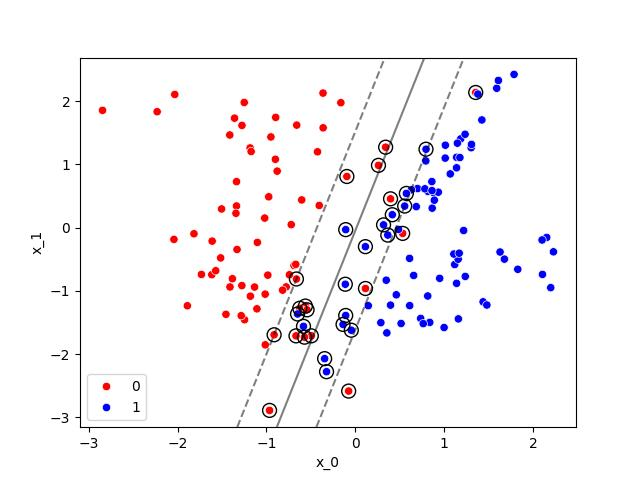
\includegraphics{figures/3_1_dataset_SVM.jpg}\\
\textbf{Figure 1. Linear SVM on Dataset}

    \hypertarget{questions}{%
\paragraph{3.1.2 Questions}\label{questions}}

For the dataset in \emph{Figure 1} there were 17 support vectors for
class 0, and 16 for class 1. If the data were linearly separable we
would expect there to be as few as a single support vector for each
class. There are cases where linearly separable classes can have more
than one support vector, but for randomly generated data with high data
percision it is unlikely to have multiple.

\emph{Figure 2} showns the effect chaning the SVM parameter \emph{C} has
on the classification accuracy. I can be clearly seen that some values
of \emph{C} produce higher accuracies for both the training and testing
set, when compared to other values. That demonstrates that choosing the
correct value of \emph{C} is important for classification performance.

\emph{Figure 2} was created using a single specific train test split. It
likely a different dataset permutation would yield a different plot.

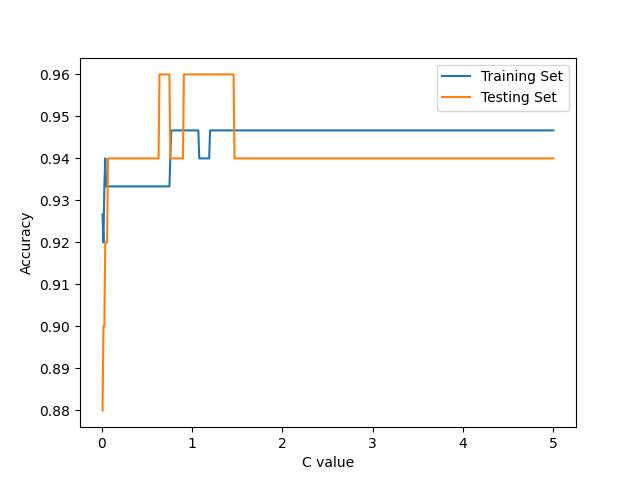
\includegraphics{figures/3_1_C_change.jpg}\\
\textbf{Figure 2. SVM C value}

The SVM returns \emph{dual coefficients}, one for each support vector
which range between values of -1 and 1. A dual coefficient with a value
of \(|\alpha_{n}| < 1\) indicates the corresponding support vector
\(x_{n}\) is a \emph{marginal} support vector, that is it lies directly
on the margin. A value \(|\alpha_{n}| = 1\) indicates the corresponding
support vector \(x_{n}\) is a \emph{non-marginal} support vector. That
is it lies off the margin at some distance in the direction of the
decision boundary. The dual vectors are bounded by -1 and 1 becuase in
the soft margin SVM formulation \(|\alpha_{n}| < C\) and in this case
\emph{C} is chosen as the default value 1.

With the \emph{dual coefficients} being known they can be used to create
the decision boundary \(g(x)\) via the following relationship.

\[
g(x) = \textbf{w}^{T}\textbf{x} + b
\] \[
\textbf{w} = \sum_{SV}{y_{n}\alpha_{n}\bf{x_{n}}}
\]

    \hypertarget{experiments}{%
\paragraph{3.1.3 Experiments}\label{experiments}}

Next consider a SVM with a polynomial kernel function. The plots of the
decision boundaries with a value of \(C=1\) can be seen in \emph{Figure
3}. The results of the classifiers with varying polynomial orders are
recorded in the following table.

\begin{longtable}[]{@{}lllll@{}}
\toprule
Order & \# \(y_{0}\) SV & \# \(y_{1}\) SV & Training Acc & Testing
Acc \\
\midrule
\endhead
2 & 70 & 70 & 0.593 & 0.540 \\
3 & 30 & 30 & 0.913 & 0.920 \\
4 & 64 & 66 & 0.586 & 0.560 \\
5 & 40 & 40 & 0.826 & 0.840 \\
\bottomrule
\end{longtable}

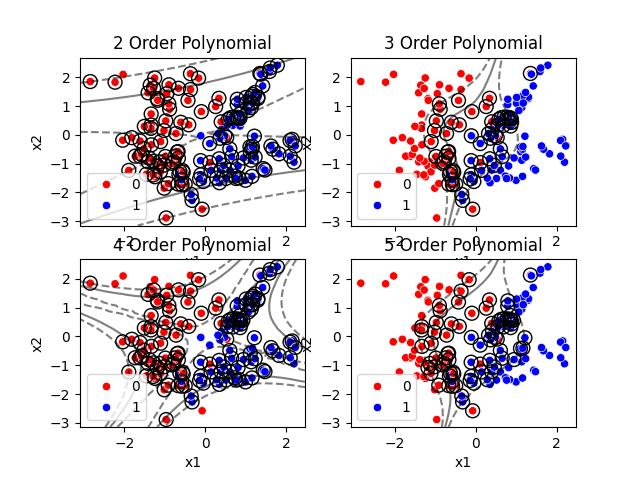
\includegraphics{figures/3_1_poly_order.jpg}\\
\textbf{Figure 3. Differing Polynomial Orders}

Clearly from the classifier accuracy the \(3^{rd}\) order polynomial
performs the best. The next investigation was to see if \(3^{rd}\) order
polynomial classifier out performing the other three was a result of the
default \emph{C} value. \emph{Figure 4} shows the results of chaning the
\emph{C} value for each order. While there is some change in the result
accuracy, the changes coming from the \emph{C} value are nowhere near
the change in accuracy as a result of order.

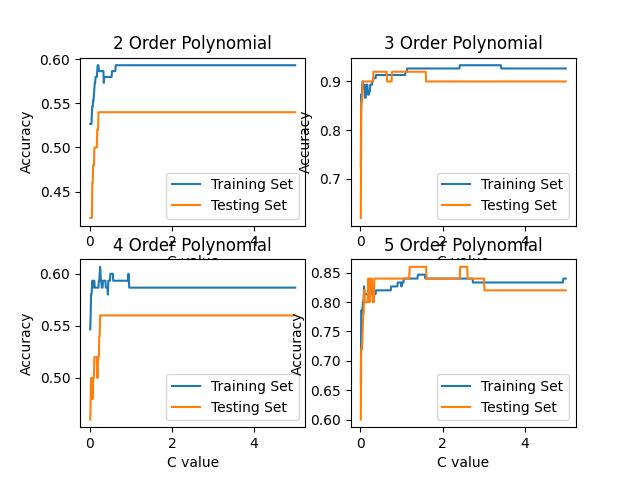
\includegraphics{figures/3_1_C_change_poly.jpg}\\
\textbf{Figure 4. Differing Polynomial Orders and C Value}

Even the best performing polynomial classifier performs worse than the
previously discussed linear classifier. It isn't too suprising given the
randomly generated dataset being used for these experiments. While it is
non-linearly separable it is very close to being which is why it would
make sense the linear classifier does such a good job.

Lastly we consider the RBF kernel function. This kernel is parameterized
by \(\gamma\). The SVC class has two default values for \(\gamma\),
\emph{auto} and \emph{scale} computed by the following equations.

\[
\gamma_{auto} = \frac{1}{d}
\] \[
\gamma_{scale} = \frac{1}{d*var(\bf{x})}
\]

Decision boundary plots for the \(\gamma_{auto}\) and \(\gamma_{scale}\)
approaches are shown in \emph{Figures 5} and \emph{6} respectively. It
can be seen that they produce very similar decision boundaries. And
perform with an accuracy nearly equivliant to that of the linear
classifer.

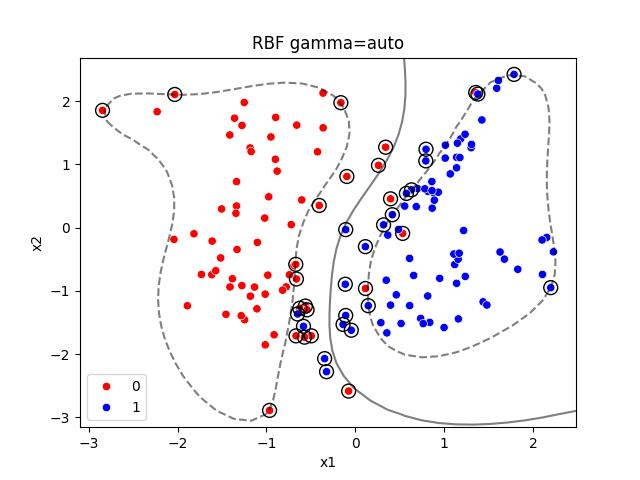
\includegraphics{figures/3_1_rbf_auto.jpg}\\
\textbf{Figure 5. Decision Boundary RBF auto}

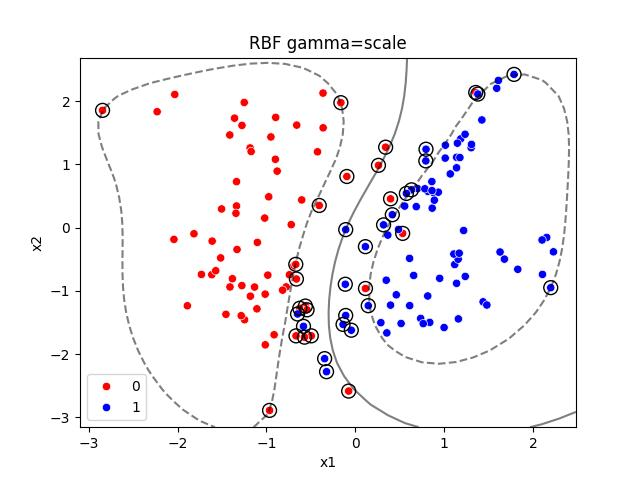
\includegraphics{figures/3_1_rbf_scale.jpg}\\
\textbf{Figure 6. Decision Boundary RBF scale}

Next to consider the effect of \(\gamma\) on the accuracy of the
classifier we again plot training and testing accuracy as a function of
the hyperparameter, in the case of RBF, \(\gamma\). It can be seen that
the \emph{auto} and \emph{scale} values of \(\gamma\) don't produce the
best result accuracy result. Being out performed by \(\gamma = 3.5\) on
both the training and testing set.

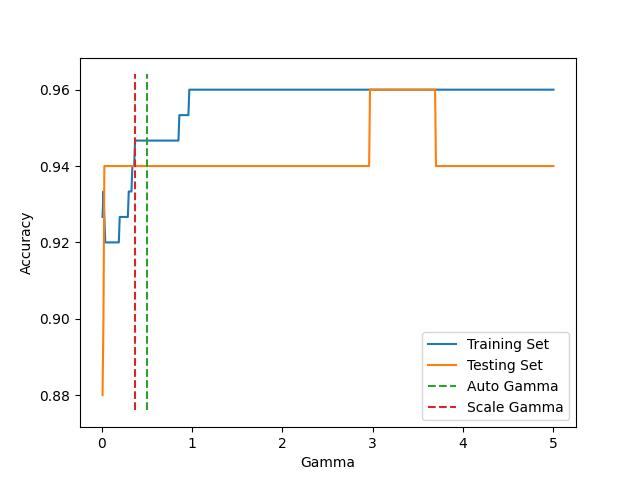
\includegraphics{figures/3_1_rbf_acc_v_gamma.jpg}\\
\textbf{Figure 7. Decision Boundary RBF scale}

If we consider the \(\gamma = 3.5\) case in \emph{Figure 8} it can be
seen that even though the accuracy is the highest for both training and
testing, the boundary is rough and the number of support vectors
drastically increases. This is an indication that this classifier is
overfit to the data, and while it performs well on this specific testing
set it will likely not acheive the same performance on a different test
set permutation.

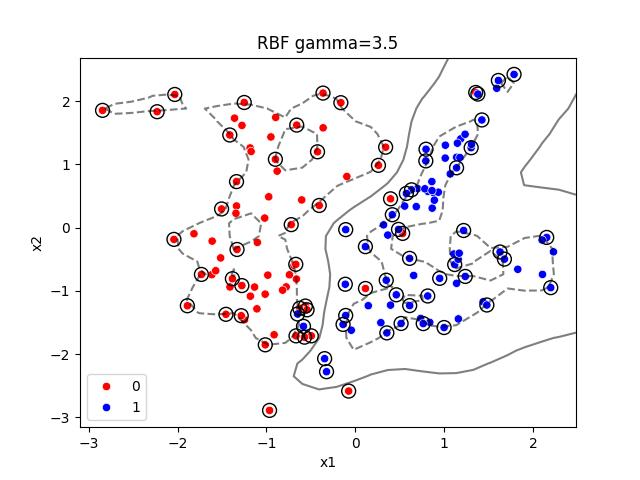
\includegraphics{figures/3_1_rbf_best.jpg}\\
\textbf{Figure 8. Decision Boundary RBF scale}

The results of the RBF investigation are summarized in tabular form
below.

\begin{longtable}[]{@{}lllll@{}}
\toprule
Gamma & \# \(y_{0}\) SV & \# \(y_{1}\) SV & Training Acc & Testing
Acc \\
\midrule
\endhead
auto & 21 & 20 & 0.946 & 0.940 \\
scale & 20 & 20 & 0.946 & 0.940 \\
3.5 & 64 & 66 & 0.960 & 0.960 \\
\bottomrule
\end{longtable}

    \hypertarget{exercise-3.2}{%
\subsection{Exercise 3.2}\label{exercise-3.2}}

The next dataset underconsideration is the \emph{Wisconsin Breast
Cancer} dataset. For this dataset each feature is on an independent
scale. As can be seen by \emph{Figure 9} when plotting the \emph{log10}
mean and variance of each feature the features can vary by multiple
orders of magnitude.

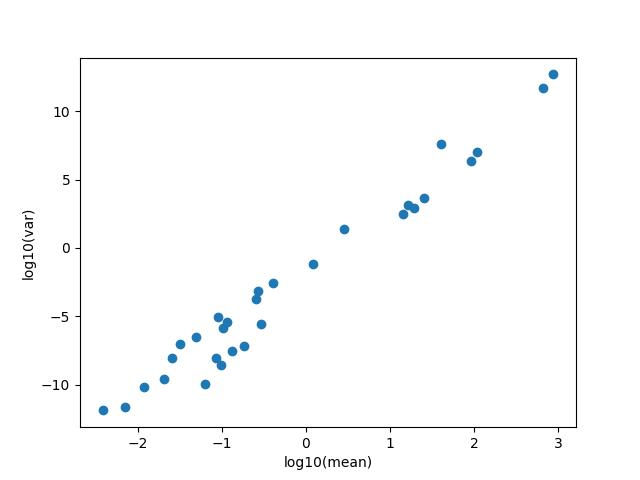
\includegraphics{figures/3_2_log_mean_var.jpg}\\
\textbf{Figure 9. Feature Log Mean Var}

SVM performs better when all the features use the same scale. For this
reason we will apply gausian normalization to each feature, which
transforms each feature from the set to have a mean of 0 and a variance
of 1. The transform is applied to each feature using the following
equation.

\[
\bf{x_{norm}} = \frac{\bf{x} - mean(\bf{x})}{var(\bf{x})}
\]

The computed mean and variance are derived only from the training data
as the held-out testing data should have no influence on how the
classifier is designed. Before running classification on the testing set
it should be transformed using the same mean and variance values
computed on the training data.

\emph{Figure 10} shows the result of this normalization transform on the
training and testing sets. As expected all the training features have a
mean of 0 and variance of 1. The testing features do not, however if we
note the linear scale of this plot verses the log scale of \emph{Figure
9}, all the features are much closer in scale than before the transform.

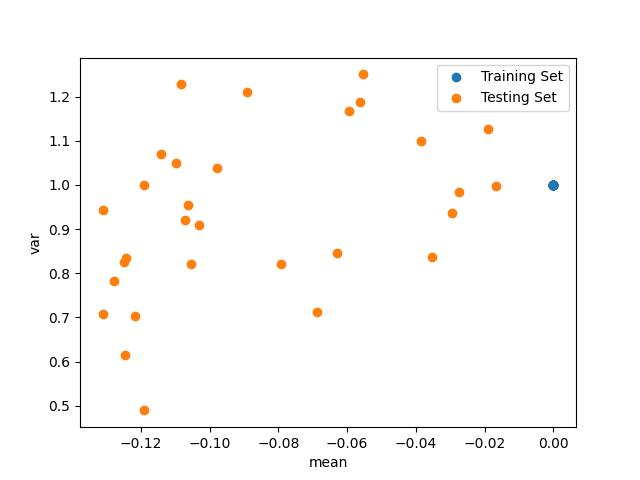
\includegraphics{figures/3_2_mean_var.jpg}\\
\textbf{Figure 10. Feature Mean Var Post Transform}

\hypertarget{experiments}{%
\paragraph{3.2.1 Experiments}\label{experiments}}

Applying a linear SVM classifier to the dataset with various values of
\emph{C} produces the results shown in the below table. It can be seen
that changing \emph{C} has a large impact on the number of support
vectors, but little impact on the accuracy of the classifer on the
held-out test set.

\begin{longtable}[]{@{}lllll@{}}
\toprule
C & \# \(y_{0}\) SV & \# \(y_{1}\) SV & Training Acc & Testing Acc \\
\midrule
\endhead
0.01 & 51 & 50 & 0.974 & 0.972 \\
0.1 & 24 & 25 & 0.988 & 0.972 \\
1 & 16 & 17 & 0.992 & 0.979 \\
10 & 13 & 14 & 0.992 & 0.979 \\
100 & 13 & 12 & 0.997 & 0.979 \\
\bottomrule
\end{longtable}

\hypertarget{experiments-1}{%
\paragraph{3.2.2 Experiments}\label{experiments-1}}

Next we applied the RBF kernel to the SVM classifier. In this case since
the training data is normalized to have a variance of 1 there is no
difference between \(\gamma_{auto}\) and \(\gamma_{scale}\). With the
default values of \(\gamma = \gamma_{scale} = \frac{1}{30}\) and
\(C = 1\), the classifier produces the results shown in the below table.

\begin{longtable}[]{@{}llllll@{}}
\toprule
C & \(\gamma\) & \# \(y_{0}\) SV & \# \(y_{1}\) SV & Training Acc &
Testing Acc \\
\midrule
\endhead
1 & 0.033 & 55 & 54 & 0.988 & 0.979 \\
\bottomrule
\end{longtable}

To visualize the effect of changing \(\gamma\) on the classifier
\emph{Figure 11} plots accuracy vs \(\gamma\). From \emph{Figure 11} it
looks like the default values of RBF do the best job. Even though
training accuracy get higher and \(\gamma\) increases the divergence
between training and testing accuracy means that data is being overfit
to the training set. The default values produces the highest accuracy on
the test set while performing similarly on both sets. As such the
default combination produces the best version of the RBF kerneled
classifier.

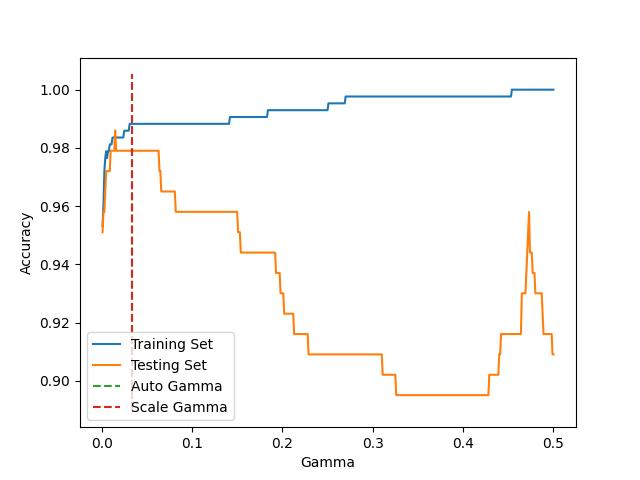
\includegraphics{figures/3_2_gamma.jpg}\\
\textbf{Figure 11. Accuracy vs \(\gamma\)}

\hypertarget{experiments-2}{%
\paragraph{3.2.3 Experiments}\label{experiments-2}}

Finally we reduce the dataset to only two features deemed important.
Using only these two features we apply the three types of kernels we've
been looking at previously and produce the following results for the
linear, \(3^{rd}\) order polynomial, and RBF kernels. Shown in
\emph{Figures 12-14} respectively.

\begin{longtable}[]{@{}lllll@{}}
\toprule
Type & \# \(y_{0}\) SV & \# \(y_{1}\) SV & Training Acc & Testing Acc \\
\midrule
\endhead
Linear & 33 & 33 & 0.955 & 0.958 \\
3rd Poly & 54 & 54 & 0.908 & 0.860 \\
RBF & 39 & 34 & 0.962 & 0.937 \\
\bottomrule
\end{longtable}

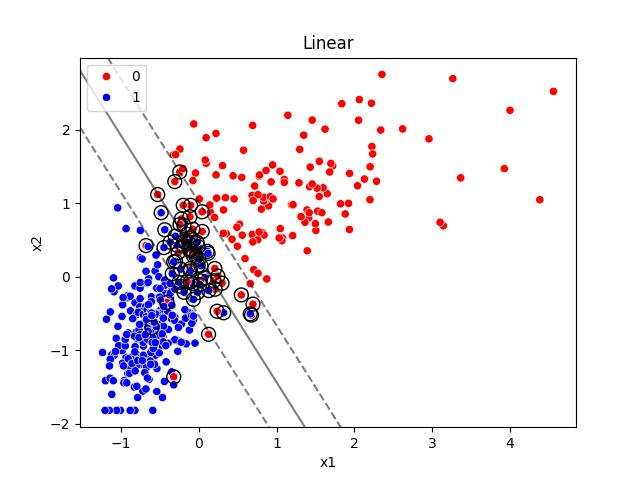
\includegraphics{figures/3_2_3_linear.jpg}\\
\textbf{Figure 12. Two Feature Linear}

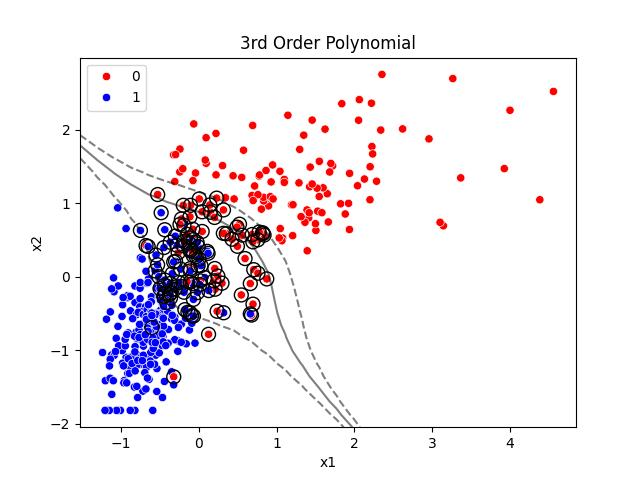
\includegraphics{figures/3_2_3_poly.jpg}\\
\textbf{Figure 13. Two Feature Polynomial}

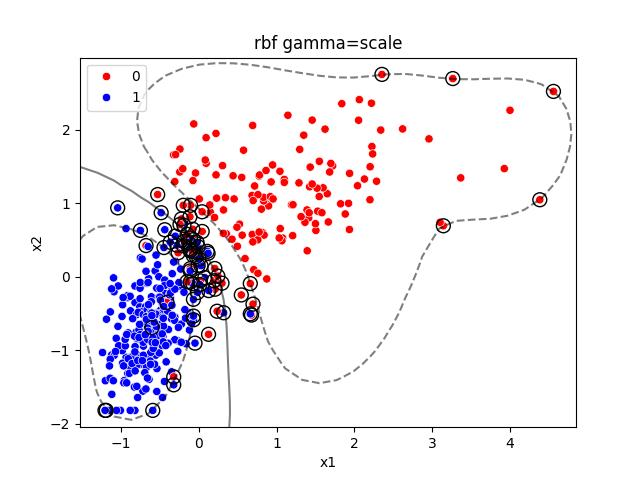
\includegraphics{figures/3_2_3_rbf.jpg}\\
\textbf{Figure 14. Two Feature RBF}

\hypertarget{final-analysis}{%
\paragraph{3.2 Final Analysis}\label{final-analysis}}

Finally of all the classifiers considered during this Experiment I would
sugguest that the 30 featured RBF kerneled classifier is the best. I
believe this to be the case for two reasons. The first being that when
considering the two feature space visualizations the decision boundary
computed by the RBF classifier appeared to be more natural to the
probable unknown truth boundary. As we have learned rarely do datasets
truely have an optimal linear boundary. Even though on the two feature
dataset the linear slightly outperformed the rbf classifier that was
only on a specific test permutation and only considering a relativly
small sample size. I think it is reasonable to make the assumption that
the decision boundary between most features tends to be more
realistically modeled by the RBF curve than a linear boundary.\\
The second reason is that for all tested classifiers the equivilant
classifier considering 30 features outperformed the two feature
counterpart. Even though the two feature classifiers performed well,
because they were consistantly out performed by the 30 feature
equivilant it leads me to believe that there is some information of
value contained in the 28 other features, and they shouldn't be
discounted even if they only add a slight improvement.


    % Add a bibliography block to the postdoc
    
    
    
\end{document}
